\documentclass{beamer}
\usetheme{Madrid}
\usepackage[T1]{fontenc}
\usepackage{mathpazo}
\usepackage{graphicx}
\usepackage{booktabs}
\usepackage{tikz}
\usetikzlibrary{positioning,arrows.meta,shapes.geometric,fit,backgrounds,calc}
\definecolor{cetnavy}{RGB}{10,26,63}
\definecolor{cetlight}{RGB}{225,231,242}
\setbeamercolor{structure}{fg=cetnavy}
\setbeamercolor{frametitle}{bg=cetnavy,fg=white}
\setbeamercolor{title}{bg=cetnavy,fg=white}
\setbeamertemplate{navigation symbols}{}
% =====================================================================
%  EDIT YOUR DETAILS HERE — this ONE file feeds every abstract & deck.
%  (Change a value, recompile; all 36 documents update.)
% =====================================================================
\newcommand{\seminarName}{Aflah Muhammed P}      % <-- your full name (guessed from your email; please verify)
\newcommand{\seminarRoll}{TVE00CS000}            % <-- your university register/roll number
\newcommand{\seminarClassRoll}{00}               % <-- your class roll no (the short one)
\newcommand{\seminarGuide}{Prof.\ <Guide Name>}  % <-- your guide
\newcommand{\seminarDept}{Department of Computer Science and Engineering}
\newcommand{\seminarCollege}{College of Engineering Trivandrum}
\newcommand{\seminarShortCollege}{CET}           % shown in the slide footer, e.g. "Aflah Muhammed P (CET)"
\newcommand{\seminarShortTitle}{B.Tech Seminar}  % middle of the slide footer
\newcommand{\seminarDate}{July 31, 2026}
% ---------------------------------------------------------------------
% Optional: put a logo image named  cet_logo.png  in this folder and it
% will appear on every title slide automatically. If absent, it is skipped.
% =====================================================================

\title[\seminarShortTitle]{SWE-Fixer: Open-Source LLMs for GitHub Issue Resolution}
\author[\seminarName\ (\seminarShortCollege)]{\seminarName \\ \seminarRoll \\ Roll No: \seminarClassRoll \\ Guide: \seminarGuide}
\institute[\seminarShortCollege]{\seminarDept \\ \seminarCollege}
\date{\seminarDate}
\titlegraphic{\IfFileExists{cet_logo.png}{\includegraphics[height=1.1cm]{cet_logo.png}}{}}
\begin{document}
\begin{frame}\titlepage\end{frame}
\begin{frame}{Table of Contents}\tableofcontents\end{frame}
\section{Introduction}
\begin{frame}{Automated GitHub Issue Resolution}
\textbf{\textit{Fixing real software, end to end}}
\begin{itemize}
\item Software maintenance means resolving issues at scale.
\item SWE-Bench: fix real GitHub issues from a repository.
\item Task: locate faulty files, then generate a patch.
\item Leading systems lean on proprietary GPT-4 / Claude.
\item Closed models limit reproducibility and access.
\end{itemize}
\end{frame}

\section{Literature Survey}
\begin{frame}{Prior Approaches}
\begin{itemize}
\item Agent systems: SWE-Agent, AutoCodeRover -- long trajectories.
\item Pipeline systems: Agentless -- staged localize then edit.
\item Open efforts: SWE-Gym, Lingma SWE-GPT trail closed models.
\item Proprietary models dominate SWE-Bench leaderboards.
\item Code retrieval: BM25 plus learned rankers.
\end{itemize}
\end{frame}

\section{Motivation}
\begin{frame}{Why a Lean Open Pipeline}
\begin{itemize}
\item Proprietary reliance harms transparency and control.
\item Agent trajectories: many calls, high latency and cost.
\item Open models lag far behind closed systems.
\item Need: reproducible, efficient, fully open resolver.
\end{itemize}
\end{frame}

\section{Problem Statement}
\begin{frame}{The Precise Problem}
\begin{itemize}
\item Given issue text and a repository, output a correct patch.
\item Two sub-problems: which files? what edits?
\item Achieve this with open weights and minimal compute.
\item Avoid costly multi-step agent exploration.
\end{itemize}
\end{frame}

\section{Objectives}
\begin{frame}{Goals and Contributions}
\begin{itemize}
\item Build a fully open-source issue-resolution pipeline.
\item Two modules: file retrieval and code editing.
\item Restrict to roughly two model calls per issue.
\item Curate a large training set with reasoning traces.
\item Match agent-level accuracy far more efficiently.
\end{itemize}
\end{frame}

\section{Methodology Overview}
\begin{frame}{Two-Module, Two-Call Pipeline}
\begin{center}
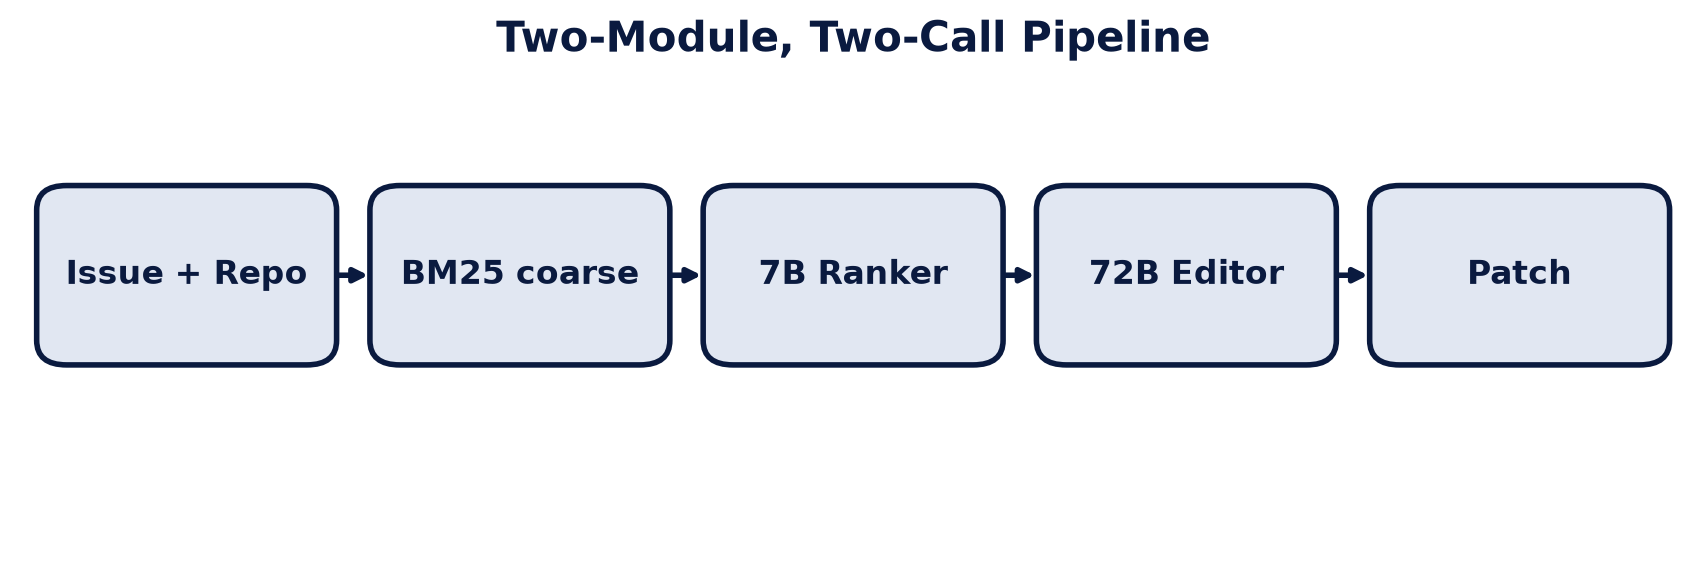
\includegraphics[width=0.9\textwidth,height=0.62\textheight,keepaspectratio]{images/swefixer_1.png}
\end{center}
\begin{itemize}
\item Retrieval call finds files; editing call writes patch.
\item Only two LLM calls, no long agent loop.
\end{itemize}
\end{frame}

\section{System Architecture}
\begin{frame}{Retrieval and Editing Modules}
\begin{center}
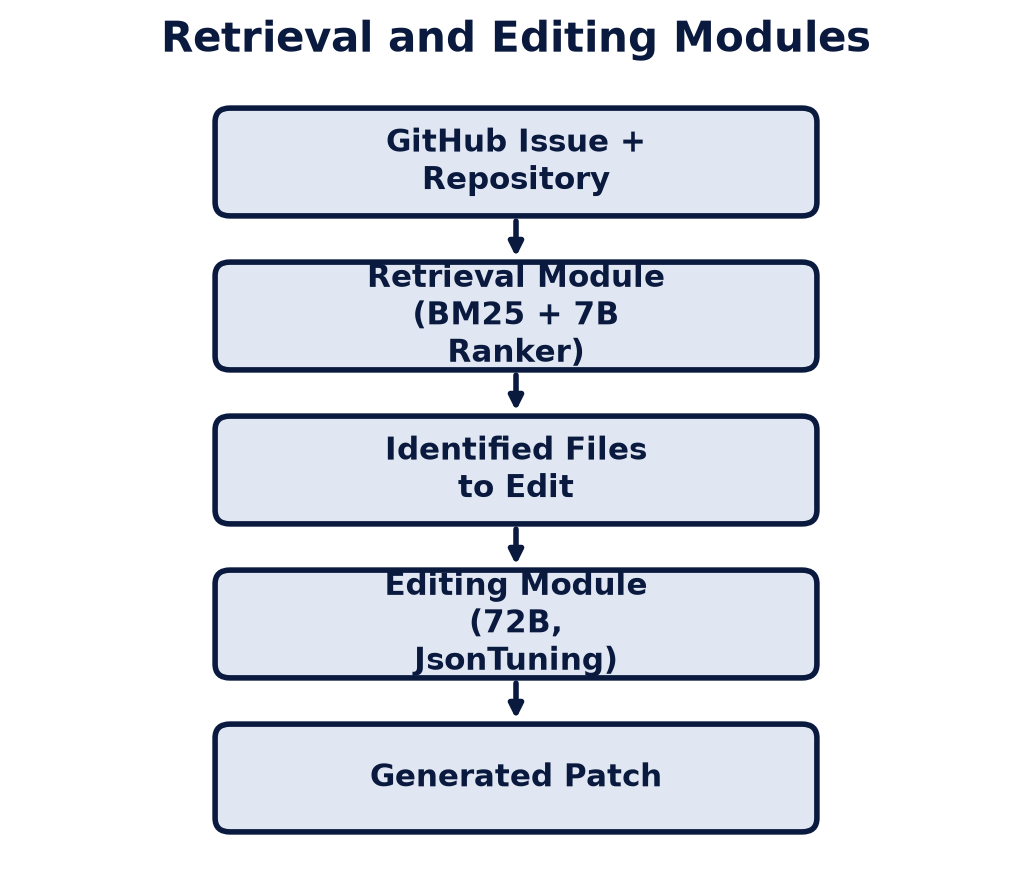
\includegraphics[width=0.9\textwidth,height=0.62\textheight,keepaspectratio]{images/swefixer_2.png}
\end{center}
\begin{itemize}
\item BM25 returns top-30 files; 7B ranker selects targets.
\item Ranker sees file skeletons: signatures and docstrings.
\item Editor consumes full files, emits structured edits.
\end{itemize}
\end{frame}

\section{Data Collection}
\begin{frame}{Building SWE-Fixer-Train-110K}
\begin{itemize}
\item Crawled 2.3K Python repos ($>$100 PRs each).
\item Collected 331K raw issue--patch instances.
\item Excluded SWE-Bench repositories to avoid leakage.
\item Dropped unparseable patches and $>$3 edited files.
\item Final corpus: 110K instances; 54.7\% single-file.
\item CoT rationales generated with GPT-4o from gold patches.
\end{itemize}
\end{frame}

\section{Model Development}
\begin{frame}{Training the Modules}
\begin{itemize}
\item Base: open Qwen2.5 series (7B retriever, 72B editor).
\item JsonTuning: structured instruction tuning format.
\item Editor output: path, original block, modified block.
\item Omits new line numbers; auto-converted to patches.
\item Retrieval trained on 80K; editing on 70K instances.
\item Resampling temperature 0 to 0.7, up to five tries.
\end{itemize}
\end{frame}

\section{Results}
\begin{frame}{SWE-Bench Verified (Best@1, \%)}
\begin{center}
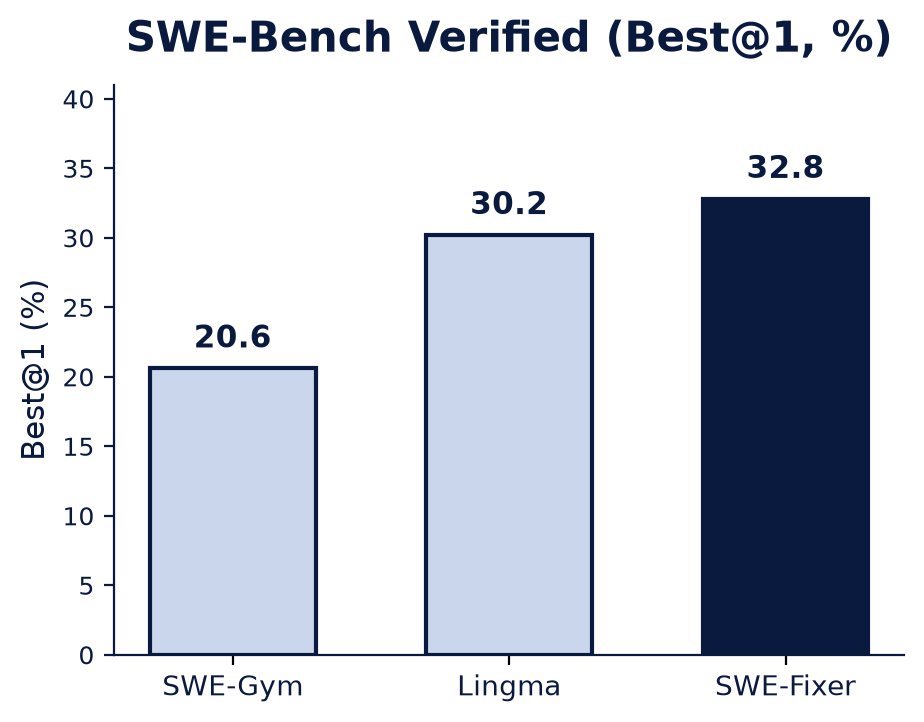
\includegraphics[width=0.9\textwidth,height=0.62\textheight,keepaspectratio]{images/swefixer_3.png}
\end{center}
\begin{itemize}
\item State-of-the-art among open-source resolvers.
\end{itemize}
\end{frame}
\begin{frame}{Headline Numbers}
\begin{center}
\begin{tabular}{lcc}
\toprule
System & Lite & Verified \\
\midrule
SWE-Gym-32B & 15.3 & 20.6 \\
Lingma-SWE-GPT-72B & 22.0 & 30.2 \\
SWE-Fixer (ours) & 24.7 & 32.8 \\
\bottomrule
\end{tabular}
\end{center}
\footnotesize
\begin{itemize}
\item Best@1 resolved \%; ours with PASS\_TO\_PASS filtering.
\item Standard scores: 22.0\% Lite, 30.2\% Verified.
\item Competitive despite only two model calls.
\end{itemize}
\end{frame}

\section{Discussions}
\begin{frame}{Why It Works}
\begin{itemize}
\item Two calls rival long, costly agent trajectories.
\item Coarse-to-fine retrieval sharpens file localization.
\item Structured edits avoid brittle line-number arithmetic.
\item CoT rationales improve reasoning over patches.
\item Weights, data, and code released openly.
\end{itemize}
\end{frame}

\section{Challenges}
\begin{frame}{Limitations}
\begin{itemize}
\item Trails Claude-3.5-Sonnet on hardest issues.
\item Compute limited editing data to 70K instances.
\item 64K context window dropped some long instances.
\item Retrieval errors cap end-to-end accuracy.
\end{itemize}
\end{frame}

\section{Future Work}
\begin{frame}{Directions Ahead}
\begin{itemize}
\item Expand training beyond 70K editing instances.
\item Reward models with Best-of-N test-time scaling.
\item Larger-scale training given more compute.
\item Extend beyond Python to more languages.
\end{itemize}
\end{frame}

\section{Conclusion}
\begin{frame}{Takeaways}
\begin{itemize}
\item SWE-Fixer: lean, open issue-resolution pipeline.
\item Retrieval plus editing in about two calls.
\item Trained on curated 110K dataset with CoT.
\item Competitive SWE-Bench Lite and Verified scores.
\item A transparent alternative to proprietary agents.
\end{itemize}
\end{frame}

\section{References}
\begin{frame}{References}
\footnotesize
\begin{itemize}
\item C. Xie, B. Li, C. Gao, et al., ``SWE-Fixer: Training Open-Source LLMs for Effective and Efficient GitHub Issue Resolution,'' arXiv:2501.05040, 2025.
\item C. E. Jimenez, J. Yang, A. Wettig, et al., ``SWE-bench: Can Language Models Resolve Real-World GitHub Issues?,'' ICLR, 2024, arXiv:2310.06770.
\item Qwen Team, ``Qwen2.5 Technical Report,'' arXiv:2412.15115, 2024.
\end{itemize}
\end{frame}
\begin{frame}\vfill\centering{\Huge Thank You}\vfill\end{frame}
\end{document}
